\documentclass{article}



\usepackage{IEEEtrantools}
\usepackage{amsmath}
\usepackage{mathrsfs}
\usepackage{graphicx}
\usepackage{subcaption}
\usepackage{setspace}
\usepackage{color}
\usepackage[margin=0.7in]{geometry}

\newcommand{\C}{\mathbf{C}}
\newcommand{\h}{\mathbf{h}}
\renewcommand{\r}{\mathbf{r}}
\newcommand{\x}{\mathbf{x}}
\newcommand{\A}{\mathbf{A}}
\newcommand{\Z}{\mathbf{Z}}
\newcommand{\Y}{\mathbf{Y}}
\newcommand{\X}{\mathbf{X}}
\newcommand{\N}{\mathcal{N}}
\newcommand{\w}{\mathbf{w}}
\newcommand{\logit}{\text{logit}}


\begin{document}

  \section{Context}

  \paragraph{NPZ model:}

  The NPZ model is the simplest meaningful model for the phytoplankton
  growth. It is a ODE model that links phytoplankton concentrations 
  (\textcolor{green}{P}) to preying zooplankton (\textcolor{red}{Z}) and
  available nutrient (\textcolor{blue}{N}) concentrations. In our case we 
  augment the NPZ model by including a nutrient flux term ($\Phi$) that 
  models an input of nutrient from the deep sea. The equations of the
  NPZ model are shown below:

  \begin{IEEEeqnarray}{rCl}
    \textcolor{green}{\frac{dP}{dt}} & = & 
    \textcolor{green}{\mu\frac{N}{k+N}P} 
    - \textcolor{red}{gPZ} 
    - \textcolor{green}{\varepsilon_PP}
    - \textcolor{green}{\varepsilon_P^* P^2},\\
    \textcolor{red}{\frac{dZ}{dt}} & = & 
    \textcolor{red}{\gamma gPZ} 
    - \textcolor{red}{\varepsilon_ZZ}
    - \textcolor{red}{\varepsilon_Z^*Z^2},\\
    \textcolor{blue}{\frac{dN}{dt}} & = &
    -\textcolor{green}{\mu\frac{N}{k+N}P} 
    + \textcolor{red}{(1-\gamma)gPZ} 
    + \textcolor{green}{\varepsilon_PP} 
    + \textcolor{red}{\varepsilon_ZZ} 
    + \Phi_N(t).
  \end{IEEEeqnarray}












  \section{Statistical modeling}

  Denote $Y_1, ..., Y_T$ the observations of chlorophyll
  concentration, $\X_1, ..., \X_T$ the state variables, with
  $\X_t = \left[N_t, P_t, Z_t, \Phi_t\right]^T$, the concentration of each of the
  ODE state variables at time $t$. For now on, we actually considere the log
  of these concentrations. 

  \begin{figure}[ht]
  \centering
    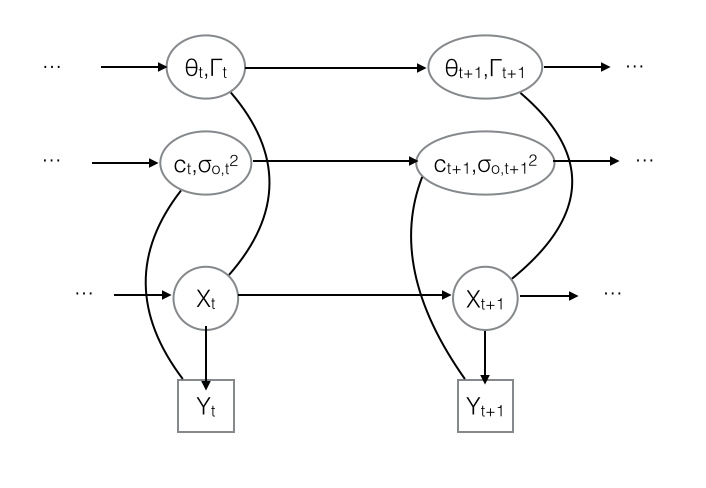
\includegraphics[scale=.3]{./BHM3.jpg}
  \caption{BHM second attempt}
  \end{figure}

  \subparagraph{Data model:}

  The observations are independent conditionally on the state of the system.

  \begin{IEEEeqnarray}{c}
  	Y_t = c_t + P_t + w^o_t,
  \end{IEEEeqnarray}

  with $w^o_t \sim \N(0, (\sigma^o_t)^2)$ iid and $c_t$ in the log-conversion
  rate between the chlorophyll and the phytoplankton concentrations. 


  \subparagraph{Process model:}

  The state variables are assumed Markovian:

  \begin{IEEEeqnarray}{c}
    X_t = \left[
      \begin{array}{c}
        N_t \\P_t\\ Z_t \\ \Phi_t
      \end{array}\right] = 
    \left[\begin{array}{c} f(X_{t-1};\theta_t)\\ \Phi_{t-1}
      \end{array}\right] + \w_t, \w_t \sim \N(0, diag(\Gamma_t))
  \end{IEEEeqnarray}

	$f$ is the result of the integration of the ODE system between times 
	$t-1$ and $t$ with initial conditions $\left[N_{t-1}, P_{t-1}, Z_{t-1}
	\right]$ and a fixed nutrient flux $\Phi_{t-1}$. 
  $\Gamma_t = \left[(\sigma_t^N)^2, 
  (\sigma_t^P)^2, (\sigma_t^Z)^2, (\sigma_t^\Phi)^2\right]$.
  $\Phi_t$ is a random walk process. 


  \subparagraph{Transition model:}

  We denote: $\lambda_t = [\theta^T_t, \Gamma^T_t, c_t, \sigma^o_t]^T$

  We have to specify a transition model for the time-varying parameters. We choose a random walk process of the form:

  \begin{IEEEeqnarray}{c}
    \logit (\lambda^{(i)}_{t+1}) = \logit (\lambda^{(i)}_t) + v^{(i)}_t,
    \text{ if } \lambda^{(i)}_t = \gamma_t, \\
    \log (\lambda^{(i)}_{t+1}) = \log (\lambda^{(i)}_t) + v^{(i)}_t,
    \text{ otherwise},
  \end{IEEEeqnarray}

 where $v^\lambda_t$ is a iid Gaussian random error of fix variance.  








\end{document}

